\documentclass[11pt,letterpaper]{article}


\usepackage[numbers,square]{natbib}
\renewcommand\cite[1]{(\citet{#1})}
\usepackage[hmargin=0.75in]{geometry}
\usepackage{color}
\usepackage{chemarr}
\usepackage{amssymb}
\usepackage{graphicx}
\usepackage{epstopdf}
\usepackage{caption}
\usepackage{subcaption}
\usepackage{placeins}
\usepackage{gensymb}
\usepackage{array}
%\usepackage{underscore}
\newcolumntype{L}{>{\arraybackslash}m{12cm}}
\usepackage{comment}
\usepackage{enumitem}

\title{IGFEM-Curves-2D: Developer's Guide}
\author{Marcus Hwai Yik Tan}
\date{Created on January 27th, 2016. Last revised on \today}

\begin{document}
\maketitle
\section{Structure of program}
\begin{figure}[!h]
\centering
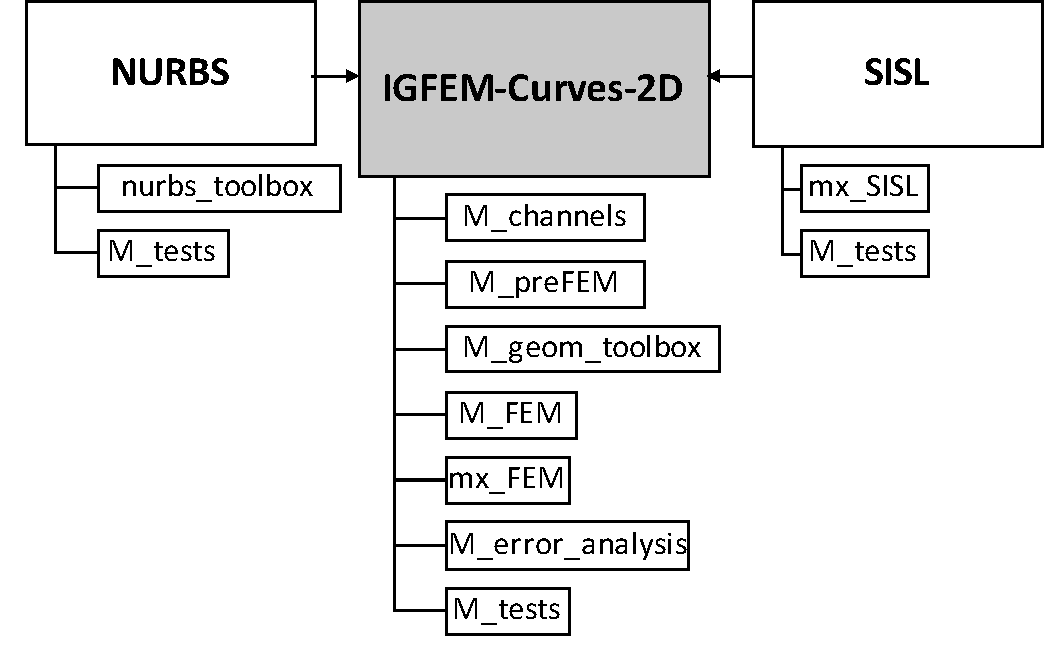
\includegraphics[width=\linewidth]{CodeStructure.pdf}
\caption{The directories (in bold) and subdirectories of the program. \label{fig_code_structure}}
\end{figure}
The program follows a straightforward functional programming paradigm. It consists of a main directory IGFEM-Curves-2D and two other directories NURBS and SISL at the same level as the main directory, as well as other subdirectories as shown in Fig.\ \ref{fig_code_structure}. The scripts are organized into subdirectories based on the types of functions they perform. Subdirectories starting with capital M  consist of MATLAB scripts while those starting with mx include MEX functions and C++ functions called by the MEX functions. The IGFEM-curves-2D directory itself contains the \texttt{main.m} script for executing the program. The other subdirectories and the types of scripts/codes located in them are described in the subsections Sec.\ \ref{subsec_M_channel} to \ref{subsec_M_error}. The subdirectories M\texttt{\_}tests in this directory as well as the other directories (NURBS and SISL) are merely directories that contain MATLAB scripts to test some MATLAB scripts or MEX functions. This is left to the developer to explore on his/her own. 

The program also needs the scripts/codes in the directories NURBS and SISL. NURBS contains a NURBS toolbox downloaded from Octave-Forge and based on the original NURBS toolbox by Mark Spink on MATLAB File Exchange. The SISL directory include MEX functions built on the SISL library developed by a group called SINTEF. Some of the MEX functions in the directory also require the Armadillo C++ lineary algebra library. The MEX functions are used for the fast calculation of intersections between common geometrical entities (such as line segment, lines etc) and NURBS or between NURBS entities. The purposes of these functions are clarified in the codes and would not be described here.  

\FloatBarrier

\subsection{IGFEM-Curves-2D/M\texttt{\_}channel}
\label{subsec_M_channel}
This subdirectory contains scripts that handle the channel networks such as:
\begin{enumerate}
\item \texttt{create\_channels\_gui.m} (creates channel input files),
\item \texttt{create\_channel.m} (an older script that create channels directly),
\item \texttt{read\_channels.m} (reads channel input file),
\item \texttt{write\_channel\_file.m} (writes channel input files ),
\item \texttt{plot\_channel\_network.m} (plots the channels, nodal pressure drops and channel flow rates),
\item \texttt{network\_pressure\_mass\_flow\_rate.m} (solves for nodal pressures and channel flow rates),
\item \texttt{branching\_point.m} (finds branching points in a network automatically),
\item \texttt{kinks.m} (finds kinks in a network described by linear NURBS so that enrichment nodes can be introduced there).
\end{enumerate}
  
It also contains scripts related to the channel networks needed by the project Opt-IGFEM-2D such as:
\begin{enumerate}
\item \texttt{generate\_sample\_file.m} (generates random initial designs using a few method like Latin hypercube sampling in bounding boxes, random shuffling in bounding boxes, random generation of quads for parallel networks and random generation of vertices followed by subgraph monomorphism to connect to vertices so that the required topology is obtained),
\item \texttt{channel\_polygons.m} (constructs triangles/quads for imposing geometrical constraints), 
\item \texttt{update\_channels.m} (updates channel control points and diameters in the optimization),
\item \texttt{design\_params2channel\_params\_map.m} (maps the channel control point coordinates to the design parameters),
\item \texttt{plot\_channels\_and\_design\_parameters.m} (plots channels and design parameters). 
\end{enumerate}
 
\subsection{IGFEM-Curves-2D/M\texttt{\_}preFEM}
This subdirectory contains scripts that perform the usual preparation for FEM analysis such as:
\begin{enumerate}
\item \texttt{generate\_uniform\_mesh.m} (generates a structural mesh),
\item \texttt{set\_boundary\_conditions.m} (sets Dirichlet and Neumann boundary conditions. Note: in the event that there are enrichment nodes along a Dirichlet boundary, this script also sets up the additional equations for applying the Lagrange multiplier method).  
\end{enumerate}

It also contains scripts that prepare the required data for IGFEM analysis such as:
\begin{enumerate}
\item \texttt{single\_edge\_curves\_intersect.m} (finds intersection between a single edge and the channel network),
\item \texttt{edges\_curves\_intersect.m}  (finds intersection between all edges of the mesh and the channel network),
\item \texttt{elem\_branching\_points.m}, \texttt{elem\_kinks.m}, \texttt{kinks\_branch\_edges\_intersect.m} (handles branching points and kinks of the channel network) 
\item \texttt{element\_intersections.m} (determines intersections of all elements with the channel network based on the edge intersections),
\item \texttt{parent\_element\_nurbs.m} (determines which elements with intersections are parent elements, i.e., those that require enrichments, extract the NURBS curve segment within the parent elements, introduce enrichment nodes at branching points and kinks etc),
\item \texttt{child\_element\_nurbs.m} (subdivides each parent element into integration subdomains/child elements),
\item \texttt{child\_elem\_nurbs\_surface.m} (constructs the NURBS surface for each integration subdomain)
\item \texttt{create\_nurbs\_enrichment\_function.m}  (extracts the basis functions associated with the enrichment control points of the subdomain NURBS surfaces and use them as enrichment functions),
\end{enumerate}

There are scripts for mesh refinements/modification such as:
\begin{enumerate}
\item \texttt{elem\_sharing\_edge\_nodes.m} (calculates sparse matrix the size of number of original nodes $\times$ number of original nodes where the (i,j) and (j,i) entries are the elements sharing the edge with nodes i and j. The matrix is used for mesh refinement by bisection.)
\item \texttt{bisection.m} (refines mesh by bisecting triangular elements)
\item \texttt{flip\_edge.m} (swaps edges of a pair of triangles to avoid certain scenarios or improve mesh quality)
\end{enumerate} 

\subsection{IGFEM-Curves-2D/M\texttt{\_}geom\texttt{\_}toolbox}
This subdirectory contains more generic geometrical tools used by the scripts in M\texttt{\_}preFEM such as:
\begin{enumerate}
\item \texttt{intersect\_edges.m} (finds intersection between edges/line segments quickly),
\item \texttt{adjacency\_matrix.m} (finds adjacency matrix of the mesh),
\item \texttt{inTriangle.m} (determines if a set of points lie within or on the boundaries of a triangle within a specified tolerance. Note: inpolygon could be used but it does not allow for the specification of tolerance).  
\end{enumerate}

\subsection{IGFEM-Curves-2D/M\texttt{\_}FEM}
This subdirectory contains scripts that perform NURBS-based IGFEM or polynomial IGFEM such as:
\begin{enumerate}
\item \texttt{gauss\_points\_and\_weights.m} (provides the gauss points and weights. Note that quadratures for tri elements are stored in the script while those for quad elements are calculated using \texttt{lgwt.m}),
\item \texttt{estimate\_nff\_nfp\_npp.m} (estimates the sizes of the different partitions (free-free, free-prescribed and prescribed-prescribed) of the stiffness matrix),
\item \texttt{assemble.m} (assembles the stiffness matrix and load vector. Note that the stiffness matrix is assembled by constructing triple vectors respectively containing the row indices, the column indices and the entry values. These vectors are then fed to the sparse function to construct the sparse stiffness matrix),
\item \texttt{assemble\_prescribed\_node.m} (assembles the vector of prescribed nodal values), 
\item \texttt{force\_assemble.m} (assembles the load vector including the entries due to the Neumann BC),
\item \texttt{compute\_regular\_element.m} (computes regular element stiffness matrix),
\item \texttt{compute\_parent\_element\_nurbs.m} (computes parent element stiffness matrix when NURBS-based IGFEM is selected),
\item \texttt{compute\_polyIGFEM\_element.m} (computes parent element stiffness matrix for polynomaial IGFEM. However, it is no longer in used as assembly is done by the mex function in the mx\texttt{\_}FEM subdirectory),
\item \texttt{local\_coord.m} (calculates local coordinates in a tri/quad element given the global coordinates),
\item \texttt{shape\_funct.m} (evaluates shape functions of tri/quad elements given local coordinates),
\item \texttt{initialize.m} (maps the node number to the equation number. Presribed nodes are mapped to negative equation numbers while free nodes are mapped to positive equation numbers),
\item \texttt{streamwise\_elem\_length.m} (calculates streamwise element lengths for applying SUPG),
\item \texttt{solve\_matrix\_eqn.m}  (solves the assembled equations), 
\item \texttt{interpolate\_soln.m} (interpolates the FEM solution for direct plotting and for error analysis),
\item \texttt{update\_enrichment\_node\_value.m} (updates the enrichment node values by adding the offsets to the background values. Note that for NURBS-based IGFEM, linear interpolation is used as it is found to be sufficiently accurate for visualization).
\end{enumerate}

Many of these scripts are not used when polynomial IGFEM is selected as the assembly of the stiffness matrix and load vector is done using the MEX function \texttt{mx\_assemble\_sparse.cpp} together with other C++ codes located in the mx\texttt{\_}FEM subdirectory. 
 
\subsection{IGFEM-Curves-2D/mx\texttt{\_}FEM}
This subdirectory contains the C++ codes require to create the MEX function \texttt{mx\_assemble\_sparse.mex*} that can be called directly in MATLAB. The function only assembles the sparse stiffness matrix and the load vector but does not solve the assembled equations since the Armadillo library does not contain a sparse solver. There are two header files here: 
\begin{enumerate}
\item \texttt{armaMex.hpp} (contains functions that allow conversion of inputs and outputs to Armadillo data structures. Note that this header file is obtained from the Armadillo package),
\item \texttt{assemble.h} (contains some inline functions and function prototypes for the functions contained in the C++ codes). 
\end{enumerate}
The purposes of the C++ codes are self-explanatory from their names and are mostly similar to those of the scripts in M\texttt{\_}FEM. Only few points warrant discussion here. First, openmp can be used in \texttt{assemble.cpp} by commenting the line \texttt{omp\_set\_num\_threads(1)}.  Second, if one needs to specify an analytical form of the distributed heat source for use with polynomial IGFEM, one needs to modify the file \texttt{body\_source\_functions.cpp}. (The analytical distributed heat source for NURBS-based IGFEM is specified in the file \texttt{distributed\_heat\_source.m} located in the subdirectory M\texttt{\_}channels.) The file \texttt{conductance.cpp} is for the constant heat flux model (channels.model $==$ 2). 

\subsection{IGFEM-Curves-2D/M\texttt{\_}error\texttt{\_}analysis}
\label{subsec_M_error}
The following scripts are included in the subdirectory to calculate the $L^2$- and $H^1$- errors and norms  given a reference solution:
\begin{enumerate}
\item \texttt{error\_L2\_H1.m} (assembles the errors squared and the reference solutions norms squared in all the elements),
\item \texttt{error\_squared\_L2\_H1\_child\_element.m} (calculates the errors squared and the reference solution norms squared in a NURBS-IGFEM integration subdomain),
\item \texttt{error\_square\_L2\_H1\_regular\_element.m} (calculates the errors squared and the reference solution norms squared in a regular element),
\item \texttt{compute\_polyIGFEM\_element\_error.m} (calculates the errors squared and the reference solution norms squared in a polynomial IGFEM parent element).
\end{enumerate}


\section{Data structures}
The purpose of this section is merely to give a general idea of the type of data structure used in the program. The definitions of the variables are best found in the comments placed in the scripts/codes or inferred from the variable names. The data structures used by the program in MATLAB are simple: matrice, vector, struct, cell and various combinations of them. For example, \\
\texttt{mesh.elem.parent(.).child(.).channelNodes} is  a struct variable that contains vector members \\
(\texttt{parent(.)} and \texttt{child(.)}) with cells (\texttt{channelNodes}). 

The main variable of the program is \texttt{mesh}. Some important members of this variable are:
\begin{enumerate}
\item \texttt{edges} with some of the members as follow:
		\begin{enumerate}%[label*=\arabic*.]
				\item \texttt{edge\_nodes} (matrix of end node numbers of the edges),
				\item \texttt{itrsect} (a vector of struct variables, each containing information about the intersections of the channels with an edge).
		\end{enumerate}
\item \texttt{elem} with some of the members as follow:
		\begin{enumerate}
				\item \texttt{elem\_node} (matrix of node numbers of the elements),
				\item \texttt{elem\_edge} (matrix of edge numbers of the elements),
				\item \texttt{junc} (a vector of struct variables the size of the number of elements containing information about branching points when applicable),
				\item \texttt{kinks} (a vector of struct variables the size of the number of elements containing information about kinks when applicable),
				\item \texttt{parent} (a vector of struct variables the size of the number of elements containing information about the enrichment nodes, channel number, integration subdomains etc when the element corresponding to an entry is a parent element),
				\item \texttt{Neumann} (struct variable containing information about the loads on the element boundaries when applicable)
		\end{enumerate}
\item \texttt{node} with some of the members as follow:
		\begin{enumerate}
				\item \texttt{coords} (matrix of the nodal coordinates, each row corresponding to a node. The first \texttt{nOriginalNodes} entries correspond to the original nodes and the rest are the enrichment nodes),
				\item \texttt{Dirichlet} (struct variable containing information about the Dirichlet boundary conditions applied to the node),
				\item \texttt{nOriginalEnrichNode} (for polynomial IGFEM, this number is the same as the total number of nodes. However, for NURBS-based IGFEM with quadratic and higher NURBS, this number only includes both the original nodes and enrichment nodes at the intersections, branching points and kinks but does not include additional enrichment nodes introduced at interior control points).  
		\end{enumerate}
\end{enumerate} 
 
Inside \texttt{mx\_assemble\_sparse.mex*} or any of the MEX functions in the SISL directory, the data structures are simply converted into corresponding data structures available in the Armadillo library, std::vector or C variables.  No custom object is defined except those that already exist in the Armadillo library. 

\section{Future development}
The efficiency of the intersection finder can be improved by sorting the edges and channels into a tree structure. Only those within the same branch need to be check for intersections. Further speed up can be achieved by using MEX functions. 

The NURBS-IGFEM assembly can be sped up by using MEX functions. This requires the use of NURBS library such as SISL.

\FloatBarrier    
\end{document}
